\subsection{Bill of Materials}
The bill of materials for a single Aether node can be found in Figure \ref{fig:BOM_1} and Figure \ref{fig:BOM_2}. These BOMs are generated from our schematics in KiCad and list all of the major components, such as ICs, as well as all minor components, such as specific capacitors and resistors. For those passive components, we have determined a specific value for them, however, we have not yet settled on a specific part number. For that reason, the passive components are simply labeled as \texttt{R\_US} or \texttt{C\_Small}. The generated BOM also lists the estimated costs of each component, with current estimated total cost of a single Aether node being \$178.03.


\begin{figure}[H]
    \centering
    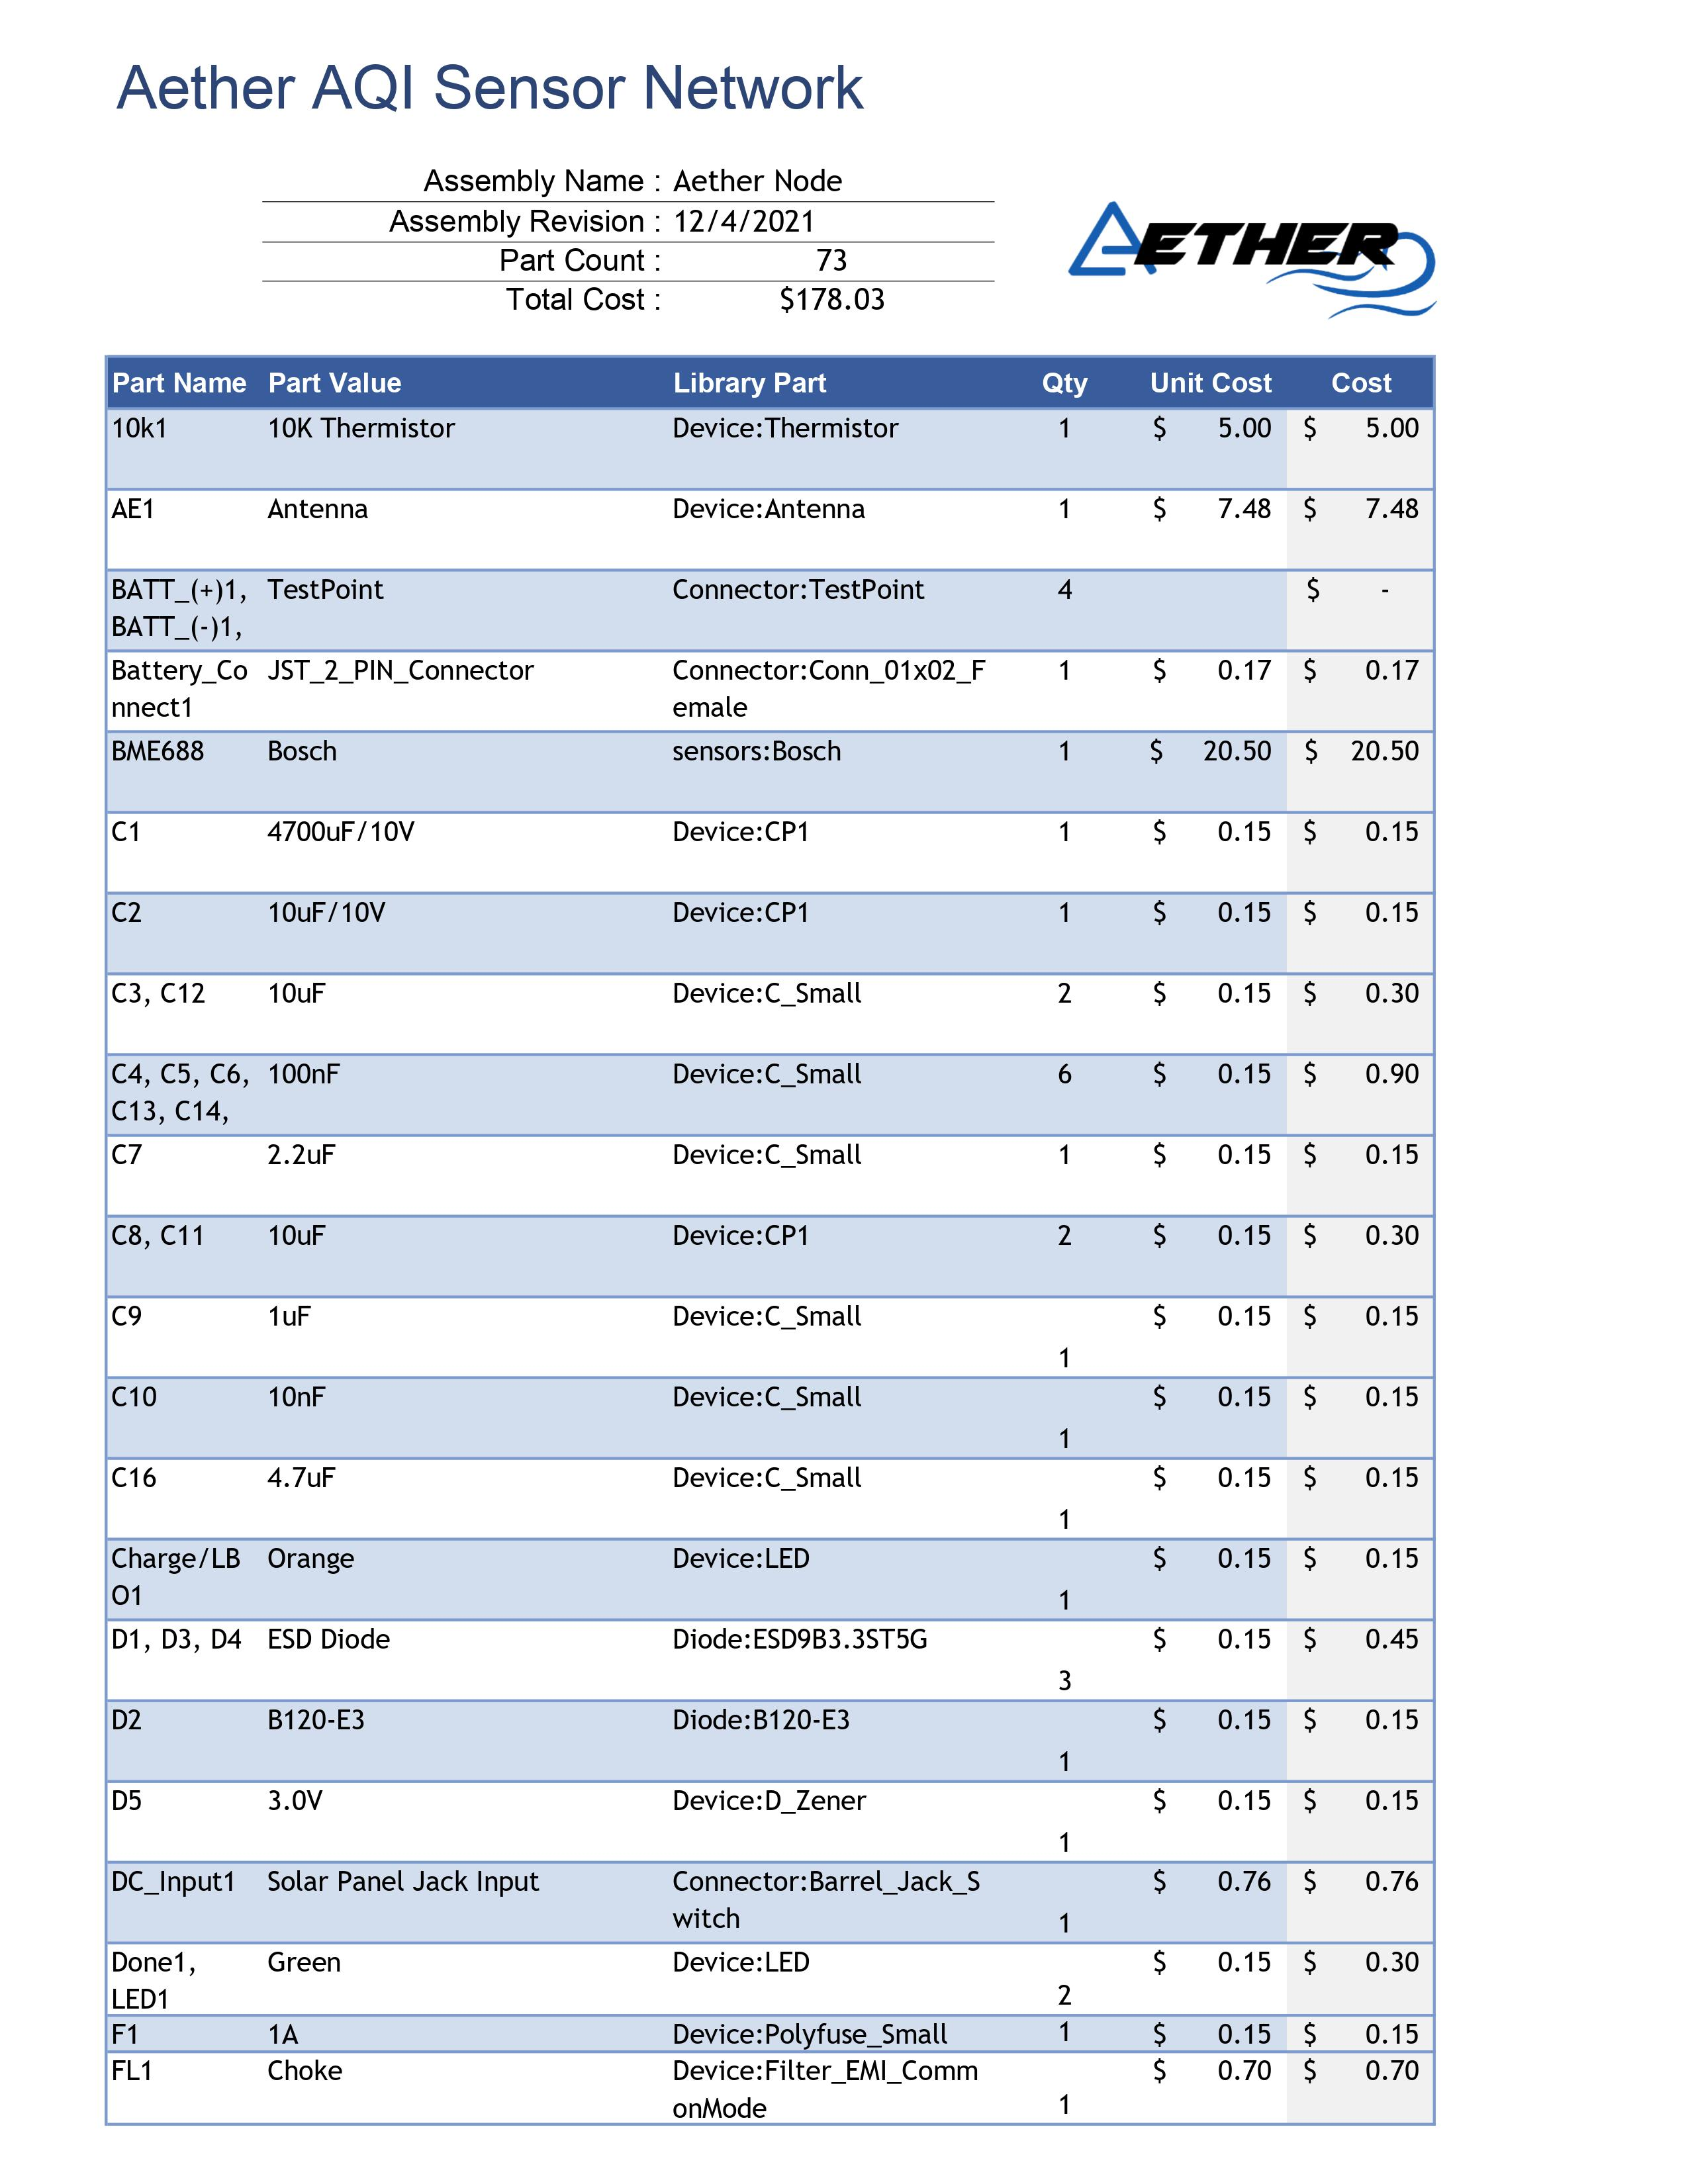
\includegraphics[width=6in]{figures/BOM_1.jpg}
    \caption{The bill of materials for a single Aether node. (Part 1)}
    \label{fig:BOM_1} 
\end{figure}

\begin{figure}
    \centering
    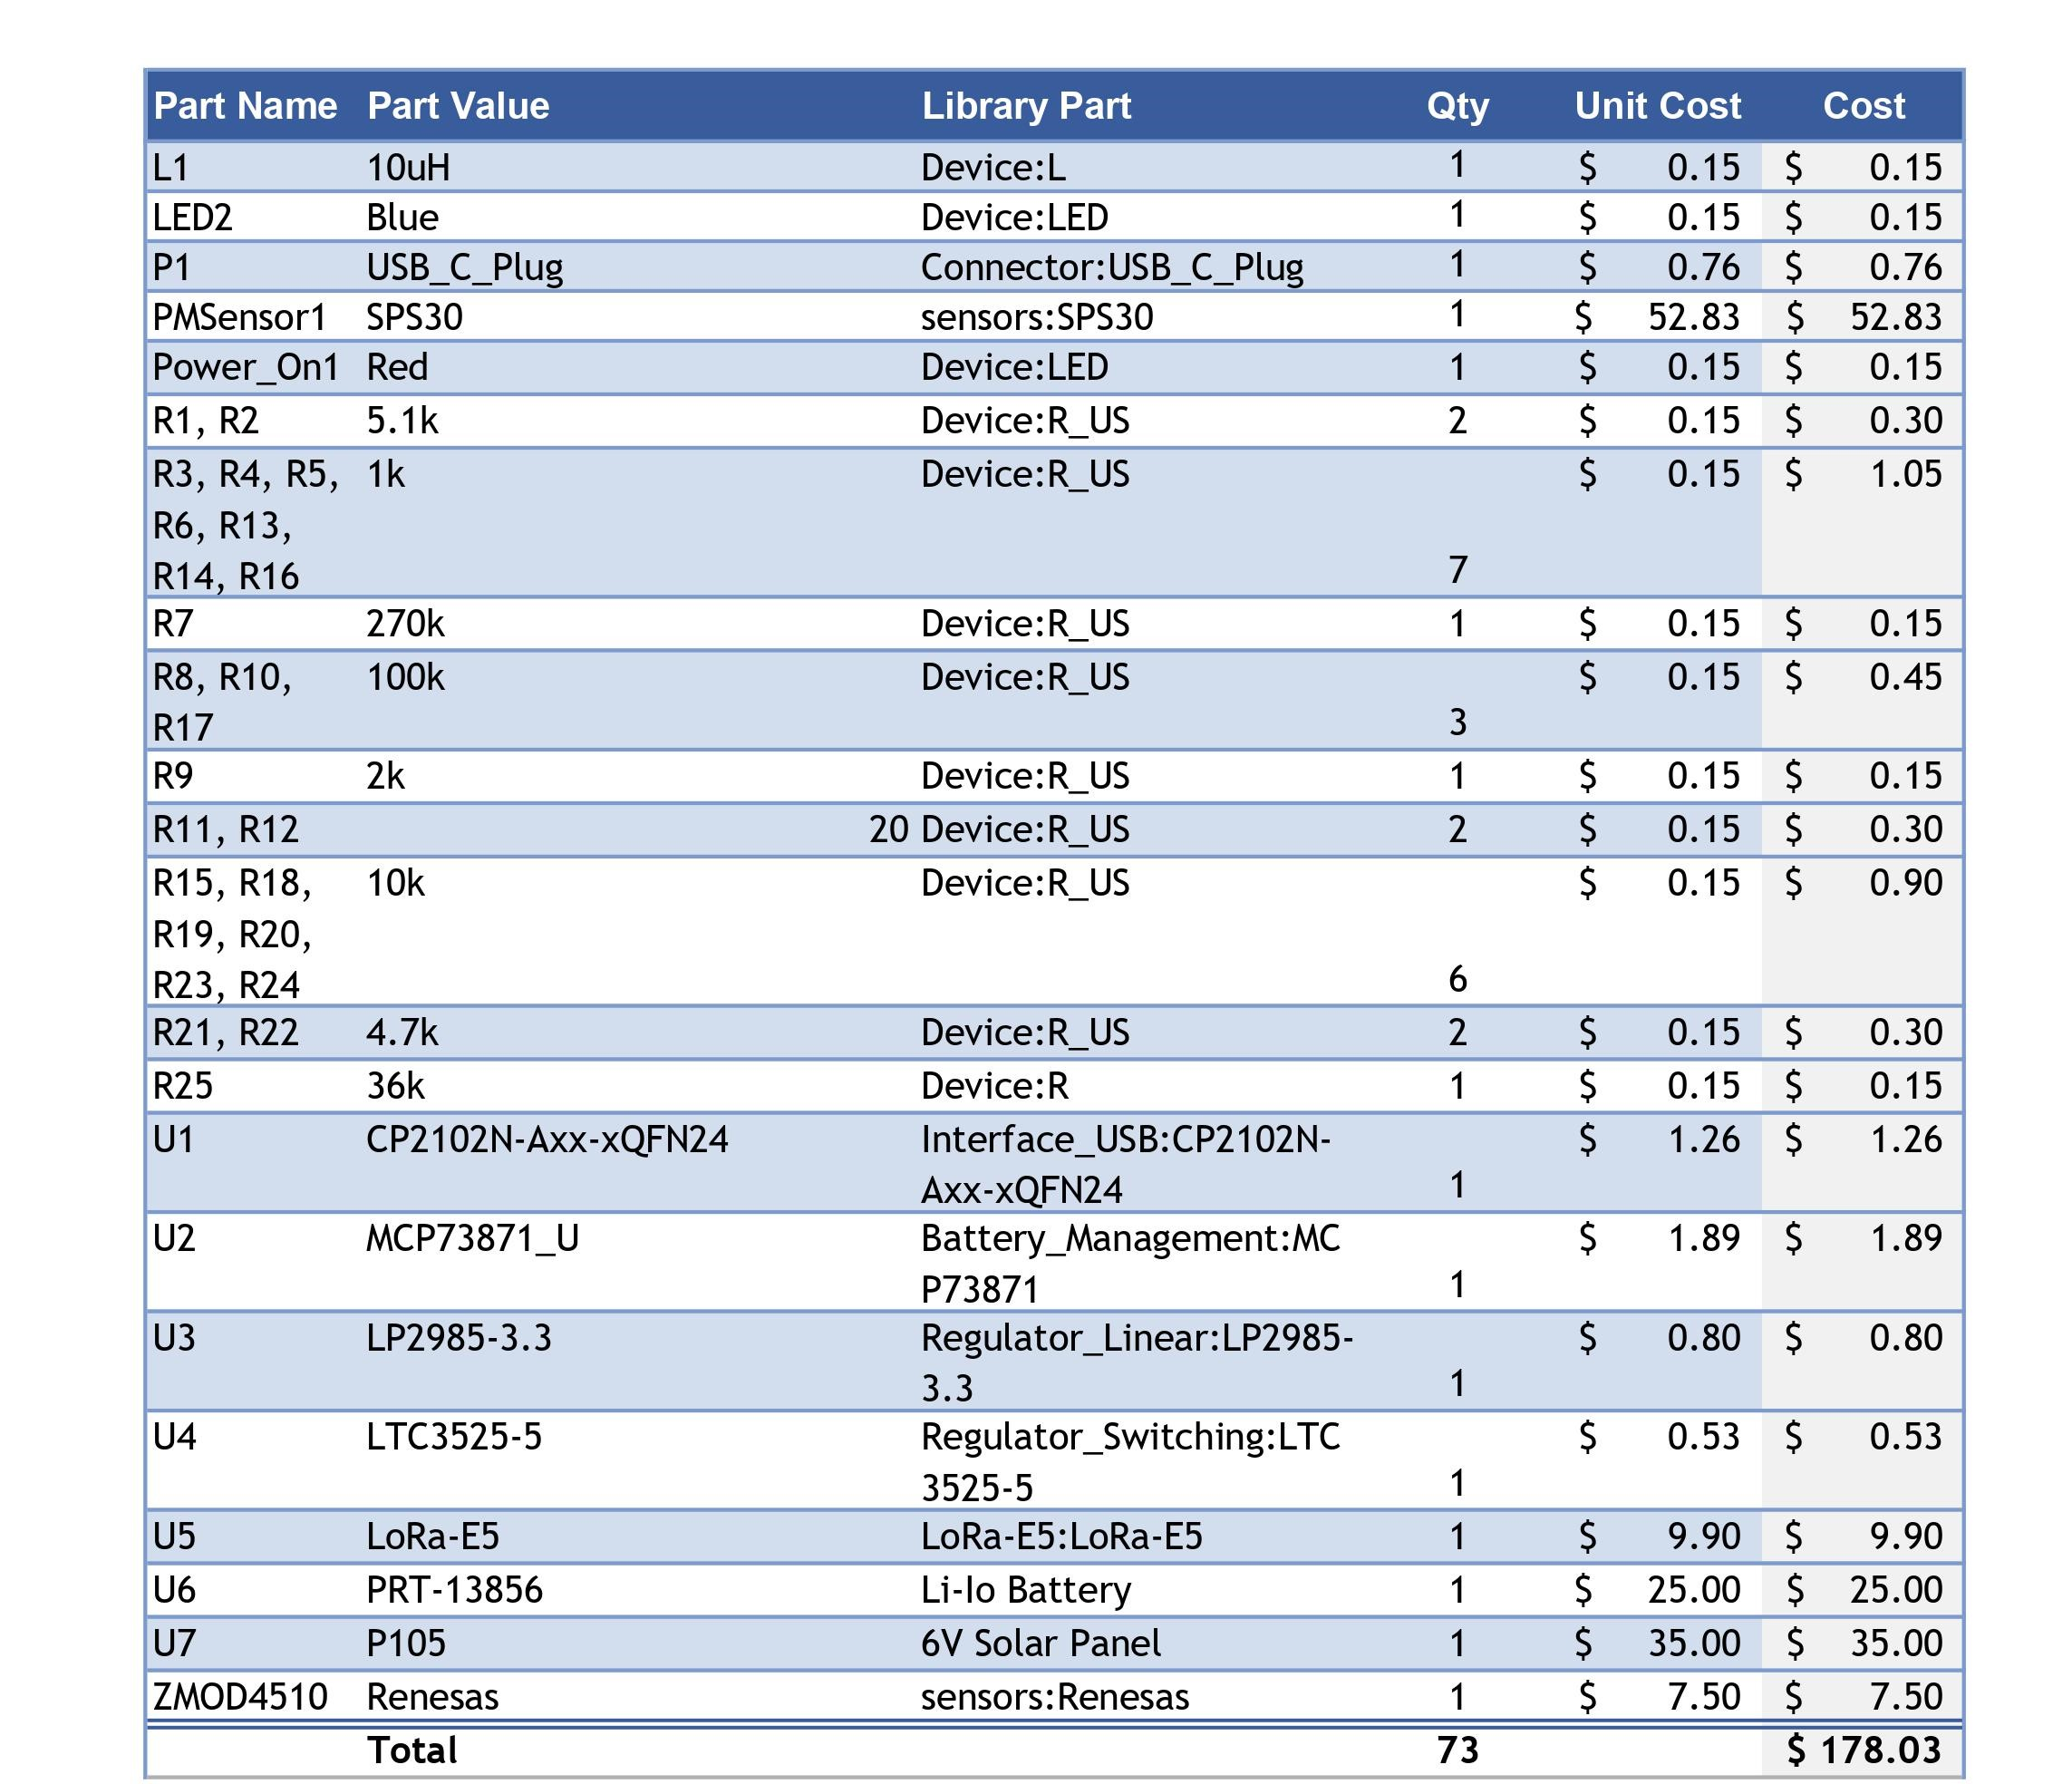
\includegraphics[width=6in]{figures/BOM_2.jpg}
    \caption{The bill of materials for a single Aether node. (Part 2)}
    \label{fig:BOM_2} 
\end{figure}